\documentclass{article}
\usepackage{amsmath,amssymb,graphicx,algpseudocode,algorithm,amsthm}
\usepackage[margin=1in]{geometry}
\usepackage{mathrsfs}
\let\mathcrl\mathscr
\usepackage[mathscr]{euscript}
\usepackage{marginnote}
\usepackage{hyperref}
\usepackage{qtree}
\usepackage{graphicx}
\usepackage{tikz}
\geometry{reversemarginpar}

\author{Benji Altman}

\def\latex{\LaTeX\ }

\newcommand{\comment}[1]{}
\def\useLim{\limits}
\newcommand{\question}[1]{\marginnote{#1}}
\let\union\cup
\let\inter\cap
\let\emptyset\varnothing
\let\bigunion\bigcup
\let\biginter\bigcap
\let\composed\circ
\let\cross\times
\def\And{\textit{ and }}
\def\Or{\textit{ or }}
\def\sbSeperator{\,\middle|\,}
\def\Return{\State\textbf{return}\par}
\def\ZNonNegative{{\mathbb Z_{\ge 0}}}
\newcommand{\setcomp}[1]{{#1}^{\mathsf{c}}}
\newcommand{\prodfrom}[3]{\prod\useLim_{#1}^{#2}\LB {#3} \RB}
\newcommand{\sumfrom}[3]{\sum\useLim_{#1}^{#2} \LB {#3} \RB}
\newcommand{\unionfrom}[3]{\bigunion\useLim_{#1}^{#2} \LB {#3} \RB}
\newcommand{\interfrom}[3]{\biginter\useLim_{#1}^{#2} \LB {#3} \RB}
\newcommand{\interacross}[2]{\interfrom{#1}{}{#2}}
\newcommand{\unionacross}[2]{\unionfrom{#1}{}{#2}}
\newcommand{\sumacross}[2]{\sumfrom{#1}{}{#2}}
\newcommand{\prodacross}[2]{\prodfrom{#1}{}{#2}}
\newcommand{\Lim}[3]{\lim\useLim_{{#1} \to {#2}}\LB {#3} \RB}
\newcommand{\set}[1]{\left\{ {#1} \right\}}
\newcommand{\setbuilder}[2]{\left\{{#1} \sbSeperator {#2}\right\}}
\newcommand{\derivative}[2]{\frac{d}{d{#2}}\LB {#1} \RB}
\newcommand{\Exists}[2]{\exists_{#1}\LB {#2} \RB}
\newcommand{\All}[2]{\forall_{#1}\LB {#2} \RB}
\newcommand{\abs}[1]{\left|{#1}\right|}
\newcommand{\card}[1]{\left| {#1} \right|}
\newcommand{\range}[1]{\textit{\textbf{Rng}}\left( {#1} \right)}
\newcommand{\domain}[1]{\textit{\textbf{Dom}}\left( {#1} \right)}
\newcommand{\pset}[1]{\mathcal P\left( {#1} \right)}
\newcommand{\pair}[2]{\left( {#1} , {#2} \right)}
\def\closure{\overline}
\newcommand{\limpts}[1]{{#1} '}
\newcommand{\ooint}[2]{\left( {#1} , {#2} \right)}
\newcommand{\ocint}[2]{\left( {#1} , {#2} \right]}
\newcommand{\coint}[2]{\left[ {#1} , {#2} \right)}
\newcommand{\ccint}[2]{\left[ {#1} , {#2} \right]}
\newcommand{\eqclass}[1]{\bar{#1}}
\newcommand{\ceil}[1]{\left\lceil {#1} \right\rceil}
\newcommand{\floor}[1]{\left\lfloor {#1} \right\rfloor}
\newcommand{\inv}[1]{{#1}^{-1}}
\def\true{\text{True}}
\def\false{\text{False}}
\newcommand{\ball}[2]{B_{#1}\left({#2}\right)}
\let\normsubgroup\triangleleft
\def\LB{}
\def\RB{}
\newcommand{\cannonicalSet}[1]{\left[ #1 \right]}
\let\lxor\oplus
\newcommand{\norm}[1]{\left|\left|{#1}\right|\right|}

\newtheorem{theorem}{Theorem}[section]
\newtheorem{lemma}[theorem]{Lemma}
\theoremstyle{definition}
\newtheorem{definition}{Definition}[section]

\input{../topology}
\usepackage[toc,xindy]{glossaries}

\makenoidxglossaries

\newglossaryentry{set}
{
	name={set},
	description={A collection of objects}
}
\newglossaryentry{vertex}
{
	name={vertex},
	description={A point or node in a graph},
	plural={vertices}
}
\newglossaryentry{edge}
{
	name={edge},
	description={A connection or line between verticies in a graph}
}
\newglossaryentry{connected}
{
	name={connected},
	description={A graph where one may start at any point and could follow edges and eventually get to any other point}
}
\newglossaryentry{multigraph}
{
	name={multigraph},
	description={Like a graph, but multiple edges may connect the same vertex pair, and an edge may connect a vertex to itself}
}
\newglossaryentry{complete}
{
	name={complete graph},
	description={A graph with all possible edges included, the notation $K_n$ is used to denote the complete with $n$ verticies}
}
\newglossaryentry{face}
{
	name={face},
	description={An section of the space we are embedding our graph in that is separated from the rest of the space by edges}
}
\newglossaryentry{contraction}
{
	name={contraction},
	description={A graph operation where one removes an edge by fusing two verticies together}
}
\newglossaryentry{subgraph}
{
	name={subgraph},
	description={$A$ is a subgraph of some graph $\mathcal G$ iff you could add verticies and edges to $A$ and somehow get $\mathcal G$}
}
\newglossaryentry{graph}
{
	name={graph},
	description={A set of verticies and edges}
}

\title{Topological Graph Theory}
\begin{document}
\maketitle
\tableofcontents



\section{Introduction}
Topological graph theory is an entire field within topology and as such this paper is by no means meant to cover all of topological graph theory in any depth. This paper instead will first cover a rather shallow overview of the field, followed by a more in depth study of graphs and their genus. The overview will mainly be focused on giving a thorough understanding of what topological graph theory is as well as to briefly cover the history of the field. In giving an overview of the field we will cover some of the basic concepts and definitions needed for the more rigorous part of the paper. After the overview we will dive into Kuratowski's Theorem, We will go through and attempt to have an intuitive understanding of a Kuratowski's Theorem and it's proof. After proving Kuratowski's Theorem, we will continue onto talking about generalizations of the theorem and map colorings, however their coverage will be rather shallow and lacking proofs.

\section{Overview}
\subsection{Graphs}
Before we talk about topological graph theory with any level of understanding we must first understand what a \gls{graph} is.

A \gls{graph} is generally defined as a \gls{set} of \glspl{vertex} combined with a \gls{set} of \glspl{edge} between \glspl{vertex}, however here it may be more useful to think about them visually with a simple representation.

Consider first a \gls{set} of points, this may be thought of as just drawing dots on a sheet of paper. Each of these points will be called a \gls{vertex}. Now we may start drawing lines between \glspl{vertex}. Lines may cross over each other and need not be straight. There is no requirement that all \glspl{vertex} have a line going to it. Each of these lines are called an \gls{edge}. We will simply insist that no \gls{edge} connects two \glspl{vertex} and that we do not have multiple \glspl{edge} between the same pair of \glspl{vertex}.

Once we have drawn this we have a representation of a \gls{graph}. If we were to move the \glspl{vertex} around on the paper but leave them having the same \glspl{edge} (the same \glspl{vertex} are connected to the point as they were before). we would be left with the same \gls{graph}. That is to say, it doesn't mater where we put a \gls{vertex} on our sheet, the \gls{graph} exists independently of the representation we draw.

\subsection{K\"onigsberg, and it's seven bridges}

Consider the following photo-realistic drawing of the city of K\"onigsberg.

\input{Konigsberg.pdf_tex}

Now the question is, if we get to choose where we start, can we go for a stroll and cross every bridge exactly once?

I first came across this question in the 8\textsuperscript{th} grade, and it was presented to us during geometry class. While undoubtedly an interesting problem, it is quite misleading to try and think of this as a geometry problem. Instead we will try and reduce it to a \gls{graph} problem.

Let us start by thinking of every island as a \gls{vertex} and every bridge as an \gls{edge}. We find the following \gls{graph}.

\begin{center}
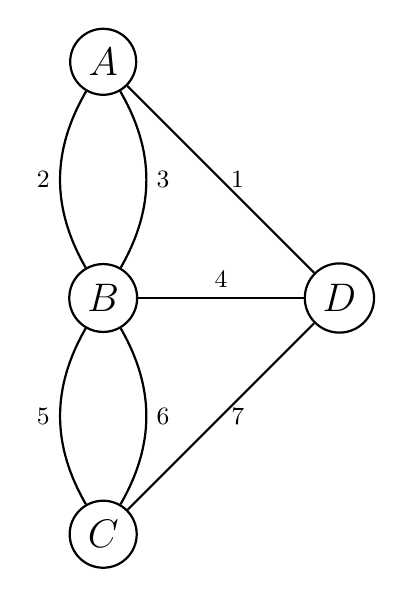
\begin{tikzpicture}[auto, node distance=3cm, every loop/.style={},
                    thick,main node/.style={circle,draw,font=\sffamily\Large\bfseries}]

  \node[main node] (1) {$A$};
  \node[main node] (2) [below of=1] {$B$};
  \node[main node] (3) [below of=2] {$C$};
  \node[main node] (4) [right of=2] {$D$};

  \path[every node/.style={font=\sffamily\small}]
    (1) edge node [right] {$1$} (4)
        edge [bend right] node[left] {$2$} (2)
    (2) edge [bend right] node [right] {$3$} (1)
        edge node {$4$} (4)
        edge [bend right] node[left] {$5$} (3)
    (3) edge [bend right] node [right] {$6$} (2)
    (4) edge node [right] {$7$} (3);
\end{tikzpicture}
\end{center}

It is worth noting two things about the above diagram. First that the labels on the \glspl{vertex} and \glspl{edge} are unrelated to the problem, but have been added simply to make referring to parts of the \gls{graph} much easier. Second that whatever the above image depicts, does not fit our definition of a \gls{graph}.

Notice that \gls{edge} $2$ and \gls{edge} $3$ both connect \gls{vertex} $A$ to $B$, as well \glspl{edge} $5$ and $6$ do for $B$ and $C$. This is a strict violation of our definition for a \gls{graph}. The issue of course then comes to what would one call such a beast as this where, presumably, one is able to have as many connections between any pair of \glspl{vertex} and could even have connections from a \gls{vertex} to itself.

I am particularly glad that you're paying enough attention to notice that the diagram does not depict a \gls{graph}. This is what we will refer to as a \gls{multigraph}. It is worth noting that \glspl{graph} are a type of \gls{multigraph}, so anything we show to be true for all \glspl{multigraph}, is also true for all \glspl{graph}.

Now to solve this problem we need to make one simple observation about how we walk. If we are to go to island (or vertex) we must also leave that island, unless it is the last island we arrive on. This means, that with the exception of the island we start on and end on, each island must have an even number of bridges connected to it. On the \gls{multigraph} we would say that we need all \glspl{vertex} but a start and end \gls{vertex} to have an even number of edges. If we look at the \gls{multigraph} above, we have four \glspl{vertex} that have an odd number of \glspl{edge} connected to them.

\subsection{History}
%TODO Make how short this is less obvious
The seven bridges of K\"onigsberg problem was solved by Euler %TODO Citation (wikipedia for seven bridges of konigsberg)
in 1736. In mathematics this problem is of great historical significance as it is considered to be the beginning of graph theory as well as a sort of precursor to topology. %TODO Citation 

\section{Graph Theory Background}

\subsection{Planer Graphs}

Consider the following \gls{graph}.

\begin{center}
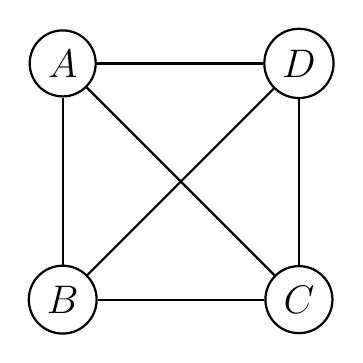
\begin{tikzpicture}[auto, node distance=3cm, every loop/.style={},
                    thick,main node/.style={circle,draw,font=\sffamily\Large\bfseries}]

  \node[main node] (1) {$A$};
  \node[main node] (2) [below of=1] {$B$};
  \node[main node] (3) [right of=2] {$C$};
  \node[main node] (4) [right of=1] {$D$};

  \path[every node/.style={font=\sffamily\small}]
    (1) edge node {} (4)
    	edge node {} (3)
    (2) edge node {} (1)
        edge node {} (4)
    (3) edge node {} (2)
    (4) edge node {} (3);
\end{tikzpicture}
\end{center}

This \gls{graph} is called a \gls{complete} as every \gls{vertex} is connected to every other \gls{vertex} by an \gls{edge}; in fact this \gls{graph} in particular is called $K_4$ as it is the complete four vertex \gls{graph}. We would like to find out if we can draw this above \gls{graph} without having any lines crossing. We can in fact draw this \gls{graph} without any intersections and for any skeptics who may being reading this, the below is $K_4$ without any \glspl{edge} intersecting.

\begin{center}
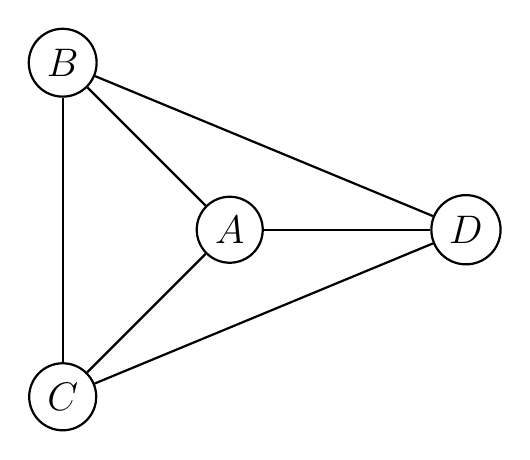
\begin{tikzpicture}[auto, node distance=3cm, every loop/.style={},
                    thick,main node/.style={circle,draw,font=\sffamily\Large\bfseries}]

  \node[main node] (1) {$A$};
  \node[main node] (2) [above left of=1] {$B$};
  \node[main node] (3) [below left of=1] {$C$};
  \node[main node] (4) [right of=1] {$D$};

  \path[every node/.style={font=\sffamily\small}]
    (1) edge node {} (4)
    	edge node {} (3)
    (2) edge node {} (1)
        edge node {} (4)
    (3) edge node {} (2)
    (4) edge node {} (3);
\end{tikzpicture}
\end{center}

So if this \gls{graph} can be drawn without intersection, can any \gls{graph} be drawn without intersections? If some can and some can't how do we tell which can be drawn and which can not? The answer to this comes in Kuratowski's theorem, however before we can even state this theorem we need to build up a bit of terminology for graph theory.

\subsection{Graph Drawing}
A graph drawing is exactly what it sounds like. We've already seen drawings of graphs like the one for K\"oingsberg and two drawings of $k_4$, this means there may be multiple distinct drawings for the same graph. Now we don't need to be very worried about what defines a drawing, that won't be important to us. Simply think of it as the drawing.

If a drawing has no edges intersecting it is said to be a plane drawing. If there exists such a drawing for a particular graph, then that graph is a planar graph.

\subsection{Face}
Faces are a bit of an odd property here as they fundamentally are actually properties only of plane drawings and not graphs themselves; however the number of faces, as we will see stays consistent between any plane drawing of a planar graph and as such the number of faces is a property that planar graphs have.

A face is defined as a connected space that contains no edges or verticies and itself is bounded by edges and verticies.

If you think back to high-school geometry and cubes you may recall that a each of the corners is a vertex, the lines connecting verticies are edges and the area between the edges are faces. In a graph we have verticies connected by edges and when we draw them there are empty areas enclosed by edges and verticies. For example the following would correspond with a cube
\begin{center}
	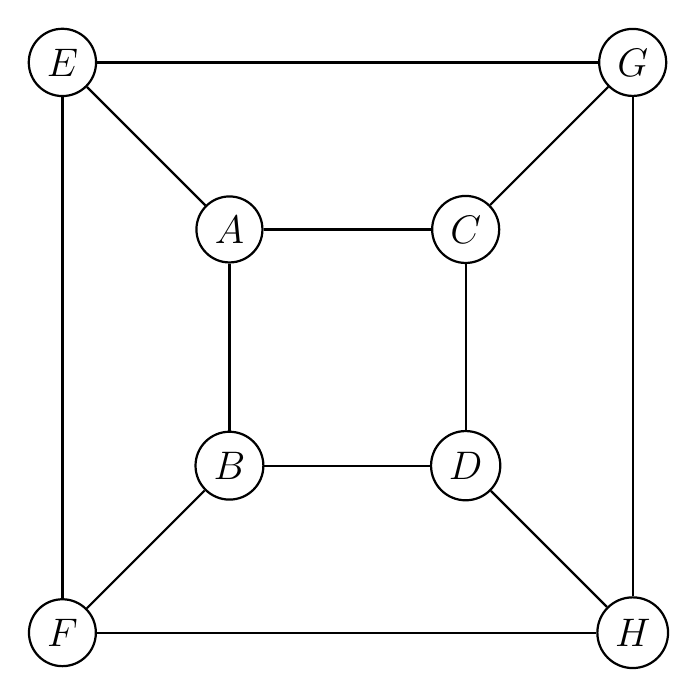
\begin{tikzpicture}[auto, node distance=3cm, every loop/.style={},
	thick,main node/.style={circle,draw,font=\sffamily\Large\bfseries}]
	
	\node[main node] (1) {$A$};
	\node[main node] (2) [below of=1] {$B$};
	\node[main node] (3) [right of=1] {$C$};
	\node[main node] (4) [right of=2] {$D$};
	\node[main node] (5) [above left of=1] {$E$};
	\node[main node] (6) [below left of=2] {$F$};
	\node[main node] (7) [above right of=3] {$G$};
	\node[main node] (8) [below right of=4] {$H$};
	
	\path[every node/.style={font=\sffamily\small}]
	(1) edge node {} (2)
	edge node {} (3)
	edge node {} (5)
	(2) edge node {} (4)
	edge node {} (6)
	(3) edge node {} (4)
	edge node {} (7)
	(4) edge node {} (8)
	(5) edge node {} (6)
	edge node {} (7)
	(6) edge node {} (8)
	(7) edge node {} (8);
	\end{tikzpicture}
\end{center}
Now we can imagine that if we look at the cube straight on maybe $ABDC$ would be the face we are looking at. So too we see the area enclosed in $ABDC$ is a face by the definition we gave. The same is true for $ABFE$, $ACGE$, $DBFH$, and $DCGH$, however that leaves us with only five faces on this cube. The last face must logically come from $EFHG$, however the area enclosed by that contains all the other edges and verticies, so it doesn't fit our definition. However we may notice that the infinite space outside $EFHG$ does not contain any verticies, and therefore we get a sixth face.

Consider then the following very simple graph:
\begin{center}
	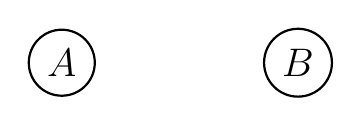
\begin{tikzpicture}[auto, node distance=3cm, every loop/.style={},
	thick,main node/.style={circle,draw,font=\sffamily\Large\bfseries}]
	
	\node[main node] (1) {$A$};
	\node[main node] (2) [right of=1] {$B$};
	
	
	\end{tikzpicture}
\end{center}
Now we still only have one face, however it doesn't have as nice a boundary as they did in the cube. However if we look at all of space excluding $A$ and $B$ then we still get a valid space by our definition.

\subsection{Path}
Now moving onto a more traditional graph property we have the concept of a path. A path is defined as a finite sequence of verticies with the property that each element of the sequence (excluding the last one) has an edge from it to the next element. For example consider the following graph.

\begin{center}
	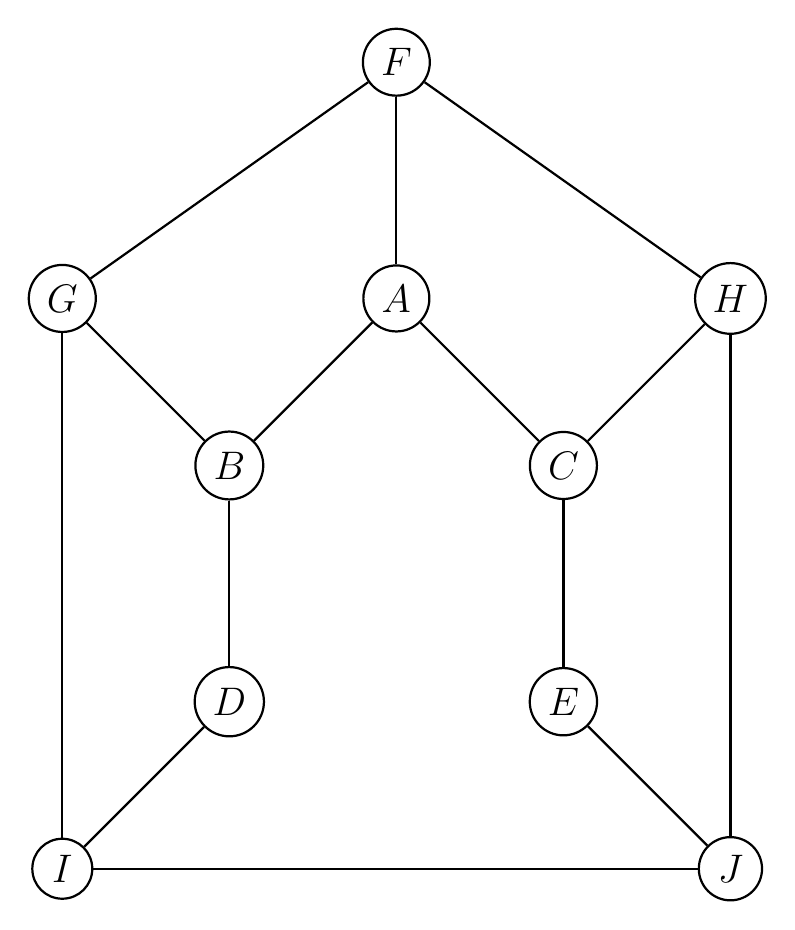
\begin{tikzpicture}[auto, node distance=3cm, every loop/.style={},
	thick,main node/.style={circle,draw,font=\sffamily\Large\bfseries}]
	
	\node[main node] (a) {$A$};
	\node[main node] (b) [below left of=a] {$B$};
	\node[main node] (c) [below right of=a] {$C$};
	\node[main node] (d) [below of=b] {$D$};
	\node[main node] (e) [below of=c] {$E$};
	\node[main node] (f) [above of=a] {$F$};
	\node[main node] (g) [above left of=b] {$G$};
	\node[main node] (h) [above right of=c] {$H$};
	\node[main node] (i) [below left of=d] {$I$};
	\node[main node] (j) [below right of=e] {$J$};
	
	\path[every node/.style={font=\sffamily\small}]
	(a) edge node {} (b)
	edge node {} (c)
	edge node {} (f)
	(b) edge node {} (d)
	edge node {} (g)
	(c) edge node {} (e)
	edge node {} (h)
	(d) edge node {} (i)
	(e) edge node {} (j)
	(f) edge node {} (g)
	edge node {} (h)
	(g) edge node {} (i)
	(h) edge node {} (j)
	(i) edge node {} (j);
	\end{tikzpicture}
\end{center}

Now the sequence $BGF$ is a path as $B$ connects to $G$ and $G$ connects to $F$. The sequence $ABGFACEJHCABA$ is also a path, however $JEDI$ is not a path as $E$ has no edge to $D$. Notice that how we draw the graph has nothing to do with what is and is not a path.

\subsection{Connected}
A graph is said to be connected if for any pair of verticies, $\pair ab$ there is a path from $a$ to $b$. So if we consider the following graphs 
\begin{center}
	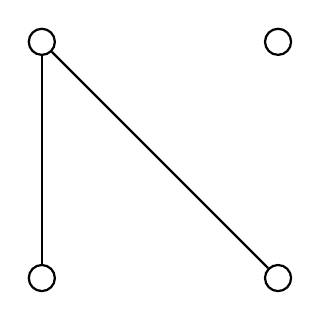
\begin{tikzpicture}[auto, node distance=3cm, every loop/.style={},
	thick,main node/.style={circle,draw,font=\sffamily\Large\bfseries}]
	
	\node[main node] (1) {};
	\node[main node] (2) [right of=1] {};
	\node[main node] (3) [below of=1] {};
	\node[main node] (4) [right of=3] {};
	
	\path[every node/.style={font=\sffamily\small}]
	(1)	edge node {} (3)
	(4) edge node {} (1);
	\end{tikzpicture}\quad\quad\quad
	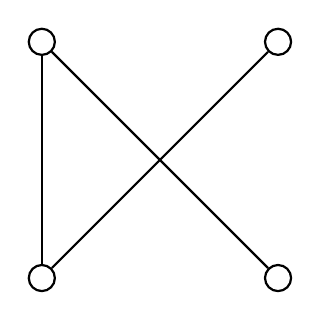
\begin{tikzpicture}[auto, node distance=3cm, every loop/.style={},
	thick,main node/.style={circle,draw,font=\sffamily\Large\bfseries}]
	
	\node[main node] (1) {};
	\node[main node] (2) [right of=1] {};
	\node[main node] (3) [below of=1] {};
	\node[main node] (4) [right of=3] {};
	
	\path[every node/.style={font=\sffamily\small}]
	(1)	edge node {} (3)
	(2) edge node {} (3)
	(4) edge node {} (1);
	\end{tikzpicture}\quad\quad\quad
	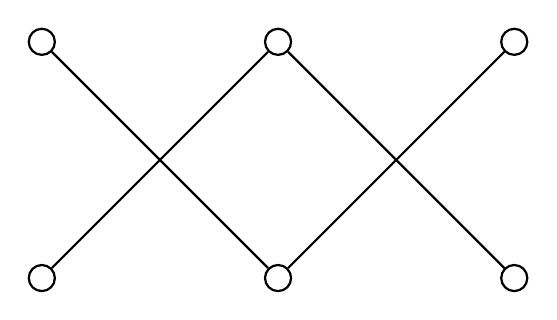
\begin{tikzpicture}[auto, node distance=3cm, every loop/.style={},
	thick,main node/.style={circle,draw,font=\sffamily\Large\bfseries}]
	
	\node[main node] (1) {};
	\node[main node] (2) [right of=1] {};
	\node[main node] (3) [right of=2] {};
	\node[main node] (4) [below of=1] {};
	\node[main node] (5) [right of=4] {};
	\node[main node] (6) [right of=5] {};
	
	\path[every node/.style={font=\sffamily\small}]
	(1)	edge node {} (5)
	(2) edge node {} (4)
	edge node {} (6)
	(3) edge node {} (5);
	\end{tikzpicture}
\end{center}
We find that only the graph in the middle is connected. For the graph on the right consider any vertex on the bottom, there is no path to the vertex above it. The graph on the left is has the upper right vertex isolated from the rest of the graph.

Any graph, connected or not, can be broken into connected components. To do this we simply take a vertex and every other vertex connected to it and call that one component, and then repeat with a vertex not in that component. This sort of breaking apart is nice as often we will prove things about connected graphs that are true about all graphs. For example if all components of a graph are planar then the entire graph must be planar, this will be proven below and it allows us to only deal with connected graphs.

\subsection{Contraction}
This is not a property, but rather an operation or action that we preform on a graph. Let us consider the following \gls{graph}.

\begin{center}
	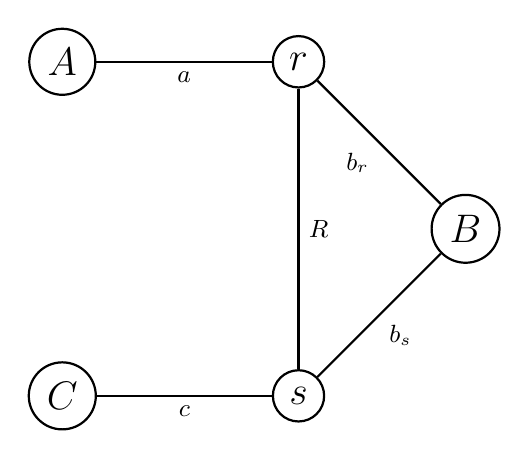
\begin{tikzpicture}[auto, node distance=3cm, every loop/.style={},
	thick,main node/.style={circle,draw,font=\sffamily\Large\bfseries}]
	
	\node[main node] (1) {$r$};
	\node[main node] (2) [below right of=1] {$B$};
	\node[main node] (3) [left of=1] {$A$};
	\node[main node] (4) [below left of=2] {$s$};
	\node[main node] (5) [left of=4] {$C$};
	
	\path[every node/.style={font=\sffamily\small}]
	(1) edge node {$R$} (4)
	edge node {$a$} (3)
	(2) edge node {$b_r$} (1)
	edge node {$b_s$} (4)
	(4) edge node {$c$} (5);
	\end{tikzpicture}
\end{center}

We wish to preform a \gls{contraction} on \gls{edge} $R$. To be clear all graph \glspl{contraction} are on \glspl{edge}. So we will make a new \gls{vertex}, $r\cdot s$ which has all the \glspl{edge} of $r$ and all the \glspl{edge} of $s$ except the \gls{edge} we are contracting across. In this case the \gls{edge} we are contracting across is $R$ and thus we get the following \gls{multigraph}.

\begin{center}
	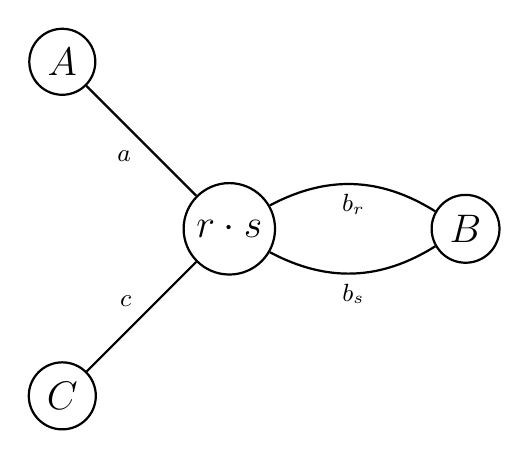
\begin{tikzpicture}[auto, node distance=3cm, every loop/.style={},
	thick,main node/.style={circle,draw,font=\sffamily\Large\bfseries}]
	
	\node[main node] (1) {$r\cdot s$};
	\node[main node] (2) [right of=1] {$B$};
	\node[main node] (3) [above left of=1] {$A$};
	\node[main node] (4) [below left of=1] {$C$};
	
	\path[every node/.style={font=\sffamily\small}]
	(1)	edge node {$a$} (3)
	(2) edge [bend right] node {$b_r$} (1)
	edge [bend left] node {$b_s$} (1)
	(4) edge node {$c$} (1);
	\end{tikzpicture}
\end{center}

This can then be reduced into a \gls{graph} again by simply treating $b_r$ and $b_s$ as the same edge. This operation is particularly important as we will prove that if a \gls{graph} is planar, then so is any \gls{graph} or \gls{multigraph} obtained by contracting an \gls{edge}.

\subsection{Subdivision}
%TODO rename unsubdivide
\def\unsubdivide{vertex replacement}
\def\unsubdividepl{vertex replacements}

To define this we first describe, we first have to describe an operation where we take a vertex $v$ that has degree 2, and replace with an edge as follows.

\begin{center}
	$
	\begin{array}{l}
		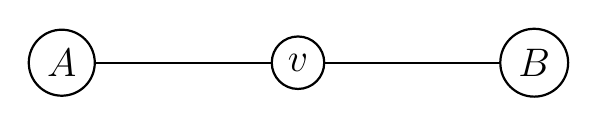
\begin{tikzpicture}[auto, node distance=3cm, every loop/.style={},
		thick,main node/.style={circle,draw,font=\sffamily\Large\bfseries}]
		
		\node[main node] (1) {$v$};
		\node[main node] (2) [left of=1] {$A$};
		\node[main node] (3) [right of=1] {$B$};
		
		\path[every node/.style={font=\sffamily\small}]
		(1)	edge node {} (2)
		edge node {} (3);
		\end{tikzpicture}
	\end{array}
	$
	\scalebox{2}{$\to$}
	$
	\begin{array}{l}
		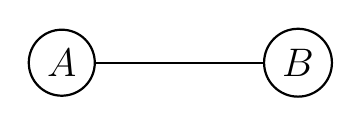
\begin{tikzpicture}[auto, node distance=3cm, every loop/.style={},
		thick,main node/.style={circle,draw,font=\sffamily\Large\bfseries}]
		
		\node[main node] (1) {$A$};
		\node[main node] (2) [right of=1] {$B$};
		
		\path[every node/.style={font=\sffamily\small}]
		(1)	edge node {} (2);
		\end{tikzpicture}
	\end{array}
	$
	
	or
	
	$
	\begin{array}{l}
		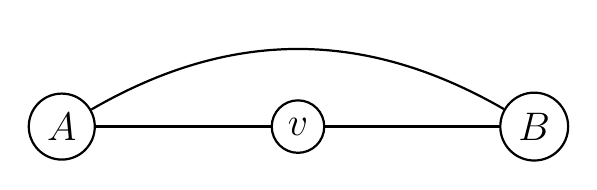
\begin{tikzpicture}[auto, node distance=3cm, every loop/.style={},
		thick,main node/.style={circle,draw,font=\sffamily\Large\bfseries}]
		
		\node[main node] (1) {$v$};
		\node[main node] (2) [left of=1] {$A$};
		\node[main node] (3) [right of=1] {$B$};
		
		\path[every node/.style={font=\sffamily\small}]
		(1)	edge node {} (2)
		edge node {} (3)
		(2) edge [bend left] node {} (3);
		\end{tikzpicture}
	\end{array}
	$
	\scalebox{2}{$\to$}
	$
	\begin{array}{l}
		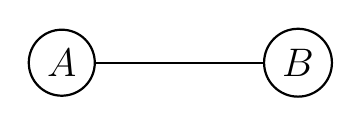
\begin{tikzpicture}[auto, node distance=3cm, every loop/.style={},
		thick,main node/.style={circle,draw,font=\sffamily\Large\bfseries}]
		
		\node[main node] (1) {$A$};
		\node[main node] (2) [right of=1] {$B$};
		
		\path[every node/.style={font=\sffamily\small}]
		(1)	edge node {} (2);
		\end{tikzpicture}
	\end{array}
	$
	
	\scalebox{.9}{Here $A$ and $B$ may be connected in any way to a larger graph, however only this subgraph will change.}
\end{center}

Now we are going to call this operation \unsubdivide, and using it we define a graph subdivision as follows.

\begin{definition}[graph subdivision]
	A graph $G$ is a subdivision of $H$ if $H$ may be produced by some series of \unsubdividepl\ on $G$.
\end{definition}

\section{Kuratowski's Theorem}
\begin{theorem}[Kuratowski's Theorem]
	A graph $G$ is nonplanar if and only if it contains a subgraph that is a subdivision of $K_{3,3}$ or $K_5$
\end{theorem}

%TODO Maybe explanation of what $K_5$ and $K_{3,3}$ are should be earlier?
Here $K_5$ refers to the complete graph on 5 vertices, and $K_{3,3}$ is the complete bipartite graph with three vertices in both partitions. Drawings of both theses graphs are below with ($K_5$ on left and $K_{3,3}$ on right).
\begin{center}
	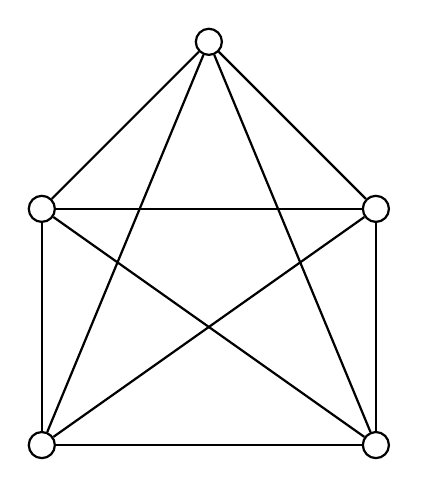
\begin{tikzpicture}[auto, node distance=3cm, every loop/.style={},
	thick,main node/.style={circle,draw,font=\sffamily\Large\bfseries}]
	
	\node[main node] (1) {};
	\node[main node] (2) [below left of=1] {};
	\node[main node] (3) [below right of=1] {};
	\node[main node] (4) [below of=2] {};
	\node[main node] (5) [below of=3] {};
	
	\path[every node/.style={font=\sffamily\small}]
	(1)	edge node {} (2)
	edge node {} (3)
	edge node {} (4)
	edge node {} (5)
	(2) edge node {} (3)
	edge node {} (4)
	edge node {} (5)
	(3) edge node {} (4)
	edge node {} (5)
	(4) edge node {} (5);
	\end{tikzpicture}
	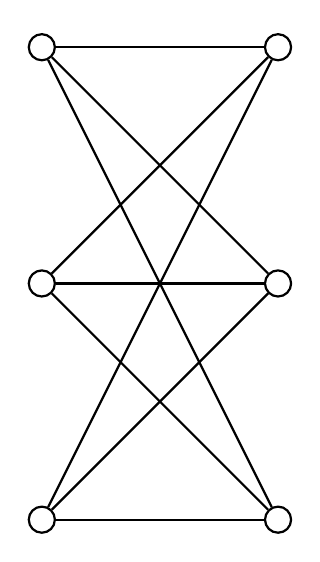
\begin{tikzpicture}[auto, node distance=3cm, every loop/.style={},
	thick,main node/.style={circle,draw,font=\sffamily\Large\bfseries}]
	
	\node[main node] (1) {};
	\node[main node] (2) [below of=1] {};
	\node[main node] (3) [below of=2] {};
	\node[main node] (4) [right of=1] {};
	\node[main node] (5) [below of=4] {};
	\node[main node] (6) [below of=5] {};
	
	\path[every node/.style={font=\sffamily\small}]
	(1)	edge node {} (4)
	edge node {} (5)
	edge node {} (6)
	(2)	edge node {} (4)
	edge node {} (5)
	edge node {} (6)
	(3)	edge node {} (4)
	edge node {} (5)
	edge node {} (6);
	\end{tikzpicture}
\end{center}

\subsection{$K_5$ and $K_{3,3}$}
Our first step is proving that $K_{3,3}$ and $K_5$ are nonplanar. To do this we are going to use the following theorem.

\begin{theorem}[Euler's formula on planar multigraphs]
	For any plane drawing of a multigraph (with the exception of a multigraph with no vertices), we have $$v-e+f=2$$, where $v$ is the number of vertices in the multigraph, $e$ is the number of edges in the multigraph, and $f$ is the number of faces in a plane drawing of the multigraph.
\end{theorem}

%TODO cite https://www.ics.uci.edu/~eppstein/junkyard/euler/iedge.html


\begin{proof}
	First consider a connected multigraph with no edges, as this is connected we may only have a single vertex. This produces a single and no edges so we find $$v-e+f=1-0+1=2$$. Now that we know that for 0 edges this rule fits, then either the rule ($v-e+f-2$) is true no mater the number of edges, or there is some number at which point this rule breaks, and $v-e+f\not=2$. If there is a number that breaks this rule, then there must be a lowest number (lets call it $k$) that breaks this rule. For any multigraph with $k$ edges, choose any edge $e$ in the graph.
	\begin{itemize}
		\item If $e$ connects a vertex to itself it is a loop and it's removal will result in the loss of one edge and one face (each loop creates a face\footnote{Jordan curve theorem}). The resulting multigraph has less than $k$ edges and thus we know that for it \begin{align*}2&=v-e+f \\&= v-(e+1)+(f+1)\end{align*} and as the original graph had one more edge and one more face it too would fit this rule.
		\item If $e$ is not a loop we may preform an edge contraction on it and this will reduce both the number of edges and the number of vertices by one. Again this gives us a multigraph with less than $k$ edges so we know that for it \begin{align*}2&=v-e+f\\&=(v+1)-(e+1)+f\end{align*} and as the original graph had one more edge and one more vertex it to would fit this rule.
	\end{itemize}
	
	From this we know that there can not possibly be some $k$, and thus all multigraphs, regardless of the number of edges must fit this rule.
\end{proof}
This leads to a nice corollary, that will be helpful when talking about graphs.
\begin{corallary}
	Any plane drawing of any multigraph has the same number of faces.
\end{corallary}
\begin{proof}
	Any planar multigraph can be broken into connected components. Each component of a planar multigraph is a connected planar multigraph and thus any planar drawing of it fits the rule $v-e+f=2$.  Now any plane drawing we make of a planar multigraph will be made of parts that already have a constant number of faces.\footnote{This is not a complete proof, to complete it you simply make an induction on the number of components drawn and realize each time you add a component you add exactly $f_{i}-1$ new faces (if $f_i$ is the number of faces in the $i^{\text{th}}$ component drawn).}
	
	%Each drawing of every component has the same number of edges and vertices, and therefore by our equation the number of faces must also be the same in each component's drawing. Now we make a plane drawing of each component one by one to create a plane drawing of the full multigraph. Choose a component to draw first and when we draw it we know it will have some number $f_1$ of faces regardless of it's drawing. Now if we have already drawn in $k$ components we can add the $k+1^{\text{th}}$ component. To do this we must draw it completely within one of the faces that already exists as it is a plane drawing. This adds exactly $f_{k+1}-1$ faces by drawing this component as it simply splits one already existing face into $f_{k+1}$ new faces. This means that no mater what order we add faces in 
\end{proof}

This means that given any planar multigraph $G$, we can talk about the number of faces $G$ has without referring to any drawing of $G$, as all plane drawings will have the same number of faces.

Now using this we can prove that $K_{3,3}$ and $K_5$ are nonplanar.

\begin{theorem}
	$K_5$ is nonplanar.
\end{theorem}
\begin{center}
	\scalebox{.6}{
		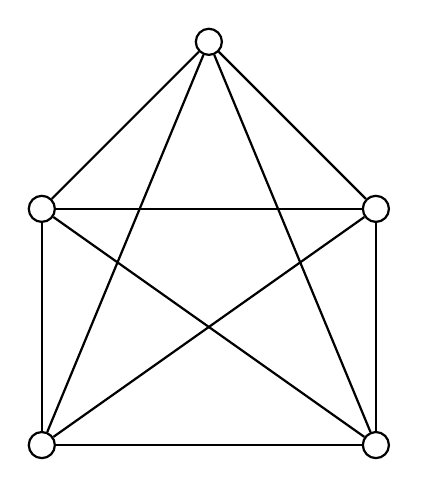
\begin{tikzpicture}[auto, node distance=3cm, every loop/.style={},
		thick,main node/.style={circle,draw,font=\sffamily\Large\bfseries}]
		
			\node[main node] (1) {};
			\node[main node] (2) [below left of=1] {};
			\node[main node] (3) [below right of=1] {};
			\node[main node] (4) [below of=2] {};
			\node[main node] (5) [below of=3] {};
			
			\path[every node/.style={font=\sffamily\small}]
			(1)	edge node {} (2)
			edge node {} (3)
			edge node {} (4)
			edge node {} (5)
			(2) edge node {} (3)
			edge node {} (4)
			edge node {} (5)
			(3) edge node {} (4)
			edge node {} (5)
			(4) edge node {} (5);
		\end{tikzpicture}
	}

	\scalebox{.9}{$K_5$}
\end{center}
\begin{proof}
	$K_5$ is a graph\footnote{Recall that all graphs are multigraphs, but not all multigraphs are graphs.}, and as such an edge can not be a loop and two vertices can share at most one edge. This means that in any plane drawing of a graph, there must be at least 3 edges bordering every face.
	\begin{itemize}
		\item To only have one edge bordering a face would require that the edge be a loop (which we can't have in a graph).
		\item To only have only two edges bordering a face would require that some pair of vertices share more than one edge (which we can't have in a graph).
	\end{itemize}
	Additionally every edge boarders no more than two faces, so from this we know that in any graph $2e \ge 3f$ or $\frac23e\ge f$. Now $K_5$ has 10 edges and 5 vertices, so we know that $$\frac2310=\frac{20}3=6.\bar6\ge f$$ We know that $K_5$ is a connected graph (and thus also a connected multigraph) so if $K_5$ were planar then we would have $$2=v-e+f=5-10+f\le5-10+6.\bar6 = 1.\bar6$$ which is clearly false as $$2\not\le1.\bar6$$ Therefore $K_5$ must not be planar.
\end{proof}

\begin{theorem}
	$K_{3,3}$ is nonplanar.
\end{theorem}
\begin{center}
	\scalebox{.6}{
		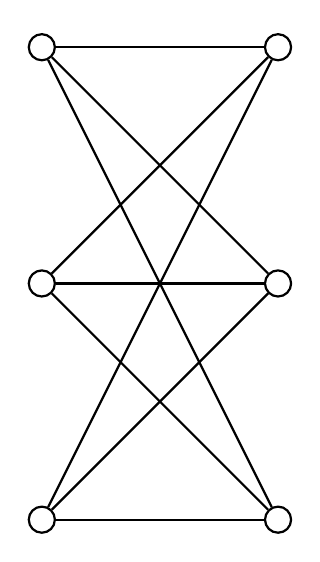
\begin{tikzpicture}[auto, node distance=3cm, every loop/.style={},
		thick,main node/.style={circle,draw,font=\sffamily\Large\bfseries}]
	
			\node[main node] (1) {};
			\node[main node] (2) [below of=1] {};
			\node[main node] (3) [below of=2] {};
			\node[main node] (4) [right of=1] {};
			\node[main node] (5) [below of=4] {};
			\node[main node] (6) [below of=5] {};
			
			\path[every node/.style={font=\sffamily\small}]
			(1)	edge node {} (4)
			edge node {} (5)
			edge node {} (6)
			(2)	edge node {} (4)
			edge node {} (5)
			edge node {} (6)
			(3)	edge node {} (4)
			edge node {} (5)
			edge node {} (6);
		\end{tikzpicture}
	}
		
	\scalebox{.9}{$K_{3,3}$}
\end{center}
\begin{proof}
	$K_{3,3}$ is a bipartite graph, meaning that there is some way to break the graph into two collections of vertices, where there are no edges that stay within one of these collections. If we look at the drawing of $K_{3,3}$ above we see that the right and left works as these collections for us. There is no edge that goes between two vertices on the right or two vertices on the left. This means that if we can make a plane drawing of $K_{3,3}$ each face must have at east four edges on it's boundary. We know from our proof of $K_5$'s nonplanarity that each face in a graph must have at least three edges on it's boundary. If any face were to have three edges then the cycle bounding the face would have exactly three vertices as well. Each pair of vertices within these three vertices would share an edge and therefore there is no way to split them up into two groups such that neither group has an edge within it. Additionally every edge boarders no more than two faces, so from this we know that in any bipartite graph $2e \ge 4f$ or $e\ge 2f$.
	
	Now $K_{3,3}$ has 6 vertices and 9 edges. $K_{3,3}$ is bipartite so the number of faces, $f \le \frac e2 = \frac92 = 4.5$. $K_{3,3}$ is connected, so if it were planar we would have Euler's formula giving us $$2=v-e+f=6-9+f\le6-9+4.5=1.5$$ and this is false as $$2\not\le1.5$$ Therefore $K_{3,3}$ is nonplanar.
\end{proof}


\printnoidxglossary

\bibliographystyle{unsrt}
\bibliography{bibliography}

\end{document}